\section{Design}
\label{sec:design}
Our design, \system{}, is based on Vizdom~\cite{vizdom} and addresses the aforementioned challenges, namely,
\begin{itemize}
    \item To formulate hypotheses via user interaction;
    \item To visualize the statistical significance and other contextual information for each observation;
    \item To control multiple hypotheses dynamically during data exploration;
    \item To progressively compute the risk of false discovery on larger data.
\end{itemize}

\subsection{Theory}
\label{sec:theory}
The theory of controlling false discovery in interactive data exploration is introduced in~\cite{zhao2016controlling}. Data exploration is treated as a growing sequence of observations.  Each observation is evaluated by a hypothesis test, which outputs a \pval{}. A false discovery procedure such as $\gamma$-Fixed~\cite{zhao2016controlling} starts with a predefined amount of exploration \textit{budget}, and \textit{invests} a fraction of the budget to each test sequentially.  If the observation is deemed significant, or equivalently, the test is rejected, then a fraction of the investment is returned to the budget. The procedure halts when either the sequence of tests stops or the budget reduces to zero.  The guarantee is that the \textit{marginalized false discovery rate} (mFDR), namely, the ratio of expected number of false discoveries over expected number of all discoveries, is less than the fraction set as the initial exploration budget.

If the exploration budget reaches zero, the per-observation investment can be reduced a posteriori for the past observations.  Because the investment corresponds to the per-test significance level, some previously significant observation may become insignificant, but because the lost of budget is also reduced.  If the reduction of investment regains eventual exploration budget, then the exploration can continue.  Such reduction policy is analogous to the Bonferroni procedure~\cite{bonferroni1936teoria}, where the significance level for each test reduces as more observations are made.

The previously known control procedures such as Bonferroni~\cite{bonferroni1936teoria}, FDR~\cite{BenjaminiH95} and Sequential FDR~\cite{g2016sequential} are not interactive, because the decisions are only finalized when all observations are made.  The main advantage of the \ainv{} procedures proposed in~\cite{zhao2016controlling} is interactivity in that observations can be made dynamically.

\subsection{User Interface}
\label{sec:ui}

\begin{figure}
\centering
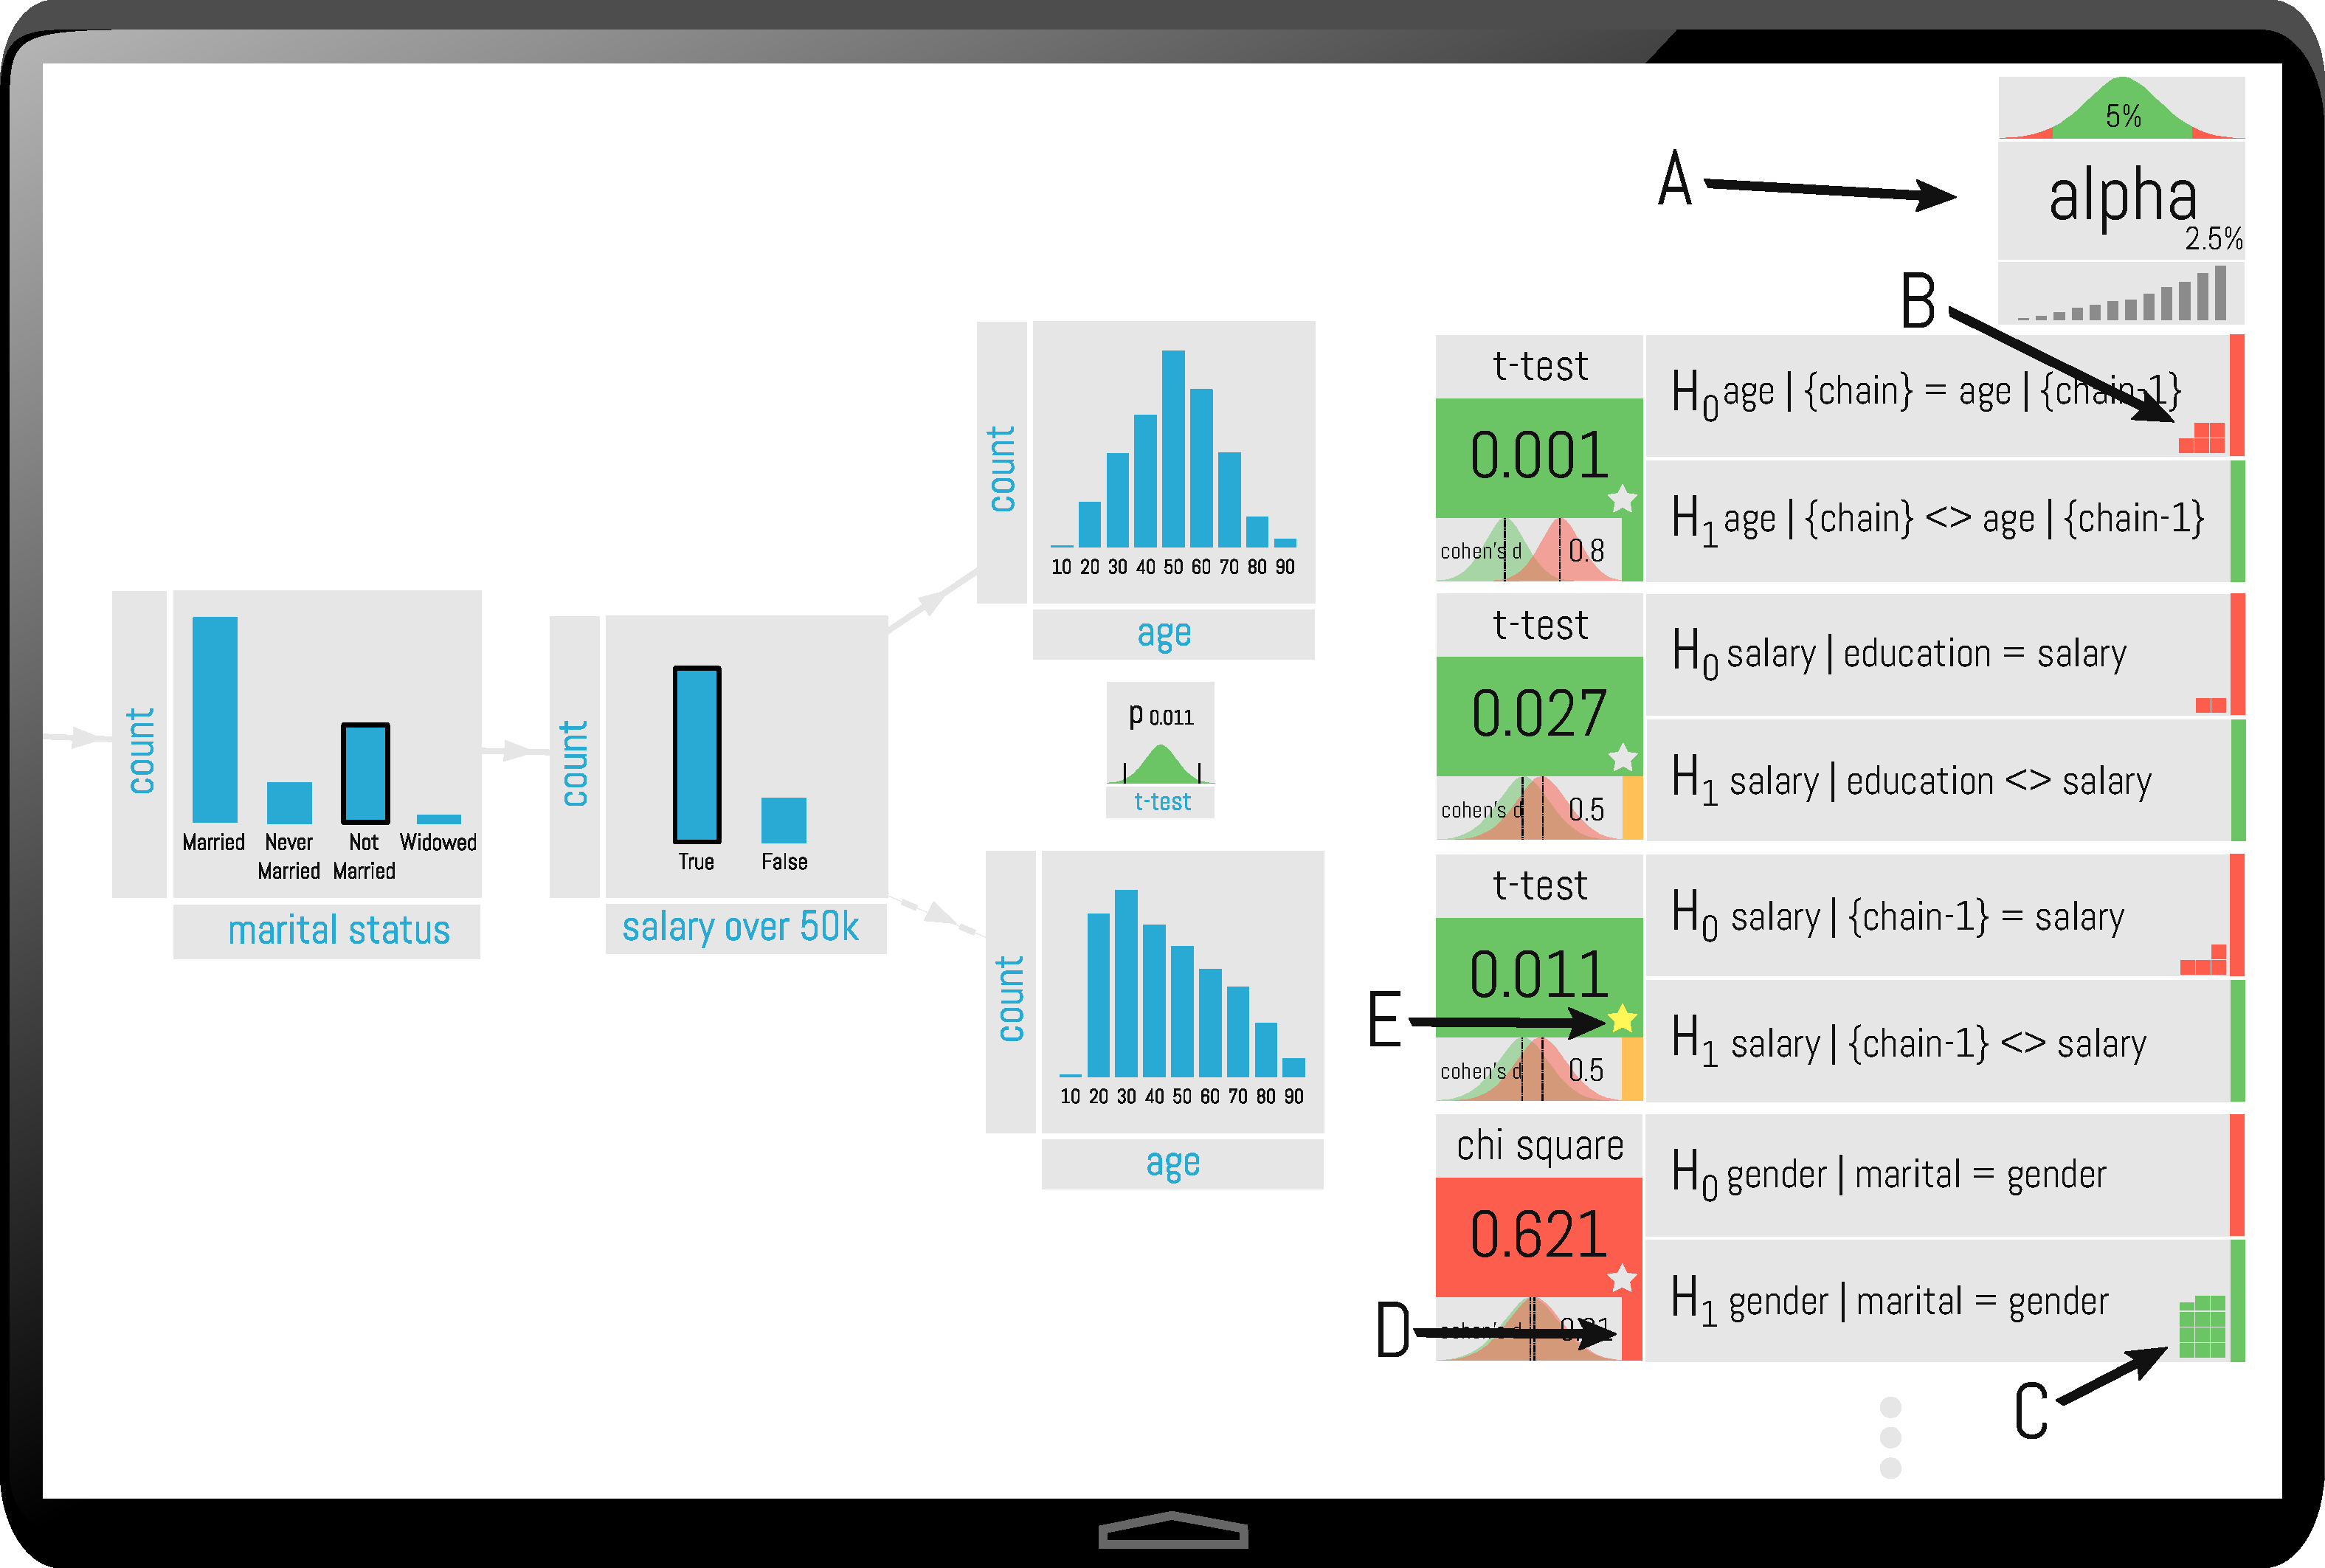
\includegraphics[width=0.47\textwidth]{figures/ui.pdf}
\caption{User Interface}
\label{fig:ui}	
\end{figure}

\system{}'s user interface (UI) features an unbounded 2D canvas where visualizations can be laid out in a free form fashion (Figure~\ref{fig:ui}). It is based on our visual data exploration tool Vizdom~\cite{vizdom} but extended by three new components:

\textbf{Explicit and implicit hypothesis testing:} For cases where users know which effect they want to verify statistically we included support to explicitly create hypothesis tests through a gestural UI that poses minimal overhead to users.
% ez: maybe talk about the automatic test selection. 
% In other cases, where users either 
% However we found that in many cases user do not deliberatly thinkg about visualizations as tests. For these instenses we ...
 
\textbf{Visualization recommendations:} To speed up the potentially laborious process of manually exploring a dataset we added a \textit{recommender}, or a visualization recommendation engine to the backend with false discovery control (Section~\ref{sec:backend}). Similar to SeeDB \cite{seedb} our engine allows users to search for filter conditions that have a significant effect (positive or negative) on a given reference visualization. We expose this functionality though a gestural touch UI that can be accessed from any visualization. 

\textbf{Hypotheses tracking:} A ``risk-gauge'' on the right-hand side of the display (A) serves two purposes, namely, to give user a summary of the multiple hypothesis correction procedure (e.g., in this case alpha investing is used with a false discovery rate of 5\% and with current remaining budget of 70\%), and to provide access to a scrollable list of all the hypotheses that have been explored.
Each list entry can be expanded (in the example all are expanded) to display details about an observation and its statistical significance.  
The text labels describe the null and alternative hypotheses for each observation and the corresponding hypothesis test and \pval{}. Each color coded tile indicates whether the observation is statistically significant or insignificant, which corresponds to green or red respectively.  
The distributions of null and alternative hypotheses and the color coded effect size are also visualized (D).  
To help the user understand the effect of data collection, the sample size estimate for the current significance level is displayed for each hypothesis test assuming the effect size is fixed (C).  
For example, the five green squares in (C) indicates approximately five times the current data size with the same effect size would make this observation significant.
Finally, important observations can be marked by tapping the ``star'' icons (E). \sam{todo: remove (B) in Figure~\ref{fig:ui}}

\subsection{Backend}
\label{sec:backend}

\begin{figure}
\centering
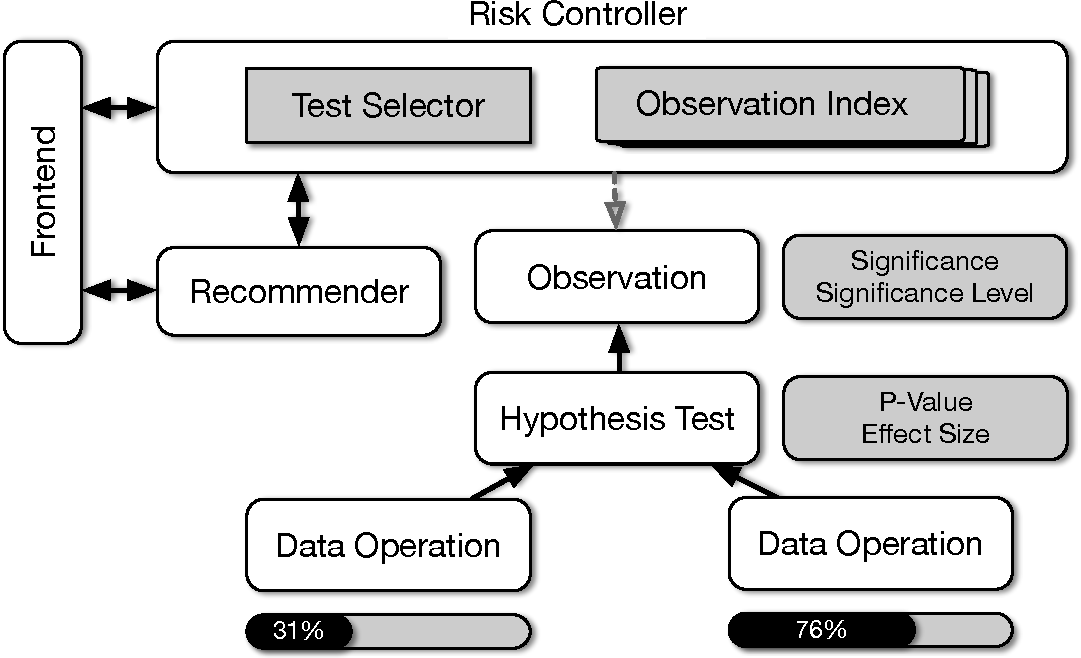
\includegraphics[scale=0.4]{figures/risk-controller.pdf}
\caption{Backend Risk Controller}
\label{fig:backend}	
\end{figure}

The highlight of the \system{} backend is the distributed and parallel computation of data-driven observations while preserving the linear ordering necessary for the false discovery procedures introduced in~\cite{zhao2016controlling}.  Our design combines functional reactive programming~\cite{wan2000functional} and progressive approximation paradigm~\cite{onlineagg,zgraggen2016progressive,vizdom} to dataflow processing to achieve practical interactivity and scalability.

The central piece of the \system{} backend is the \textit{risk controller} that implements the false discovery control procedures as introduced in~\cite{zhao2016controlling}.  Figure~\ref{fig:backend} highlights the design.  A risk controller bootstraps with a predefined exploration budget on a new dataset and invests a fraction on each observation, as described in Section~\ref{sec:theory}.  Observations are created by either the frontend user manually or the backend recommender.  Observations are tracked and indexed by the risk controller to make global decisions on each observation's appropriate significance level and its significance. A loose analogy of the observation index is perhaps a version control system, such as Git~\cite{torvalds2010git}, but in this case for data-driven observations. Such design allows distributed and parallel computation of observations for better performance, yet meanwhile enforces a linear ordering for the false discovery control procedures in~\cite{zhao2016controlling}. The observation index can also be used to look up the same observations for different frontend users or the backend recommender. 

An observation is a comparison of two distributions based on different conditions.  A comparison, for example, can be of the means, variances, correlations or histogram frequencies. Each observation is formulated as a null and an alternative hypothesis.  The risk controller is responsible of choosing the appropriate hypothesis test based on a given observation.  For example, to compare two means being different, a two-sided $t$-test is chosen; $\chi^2$-test is used to compare two histograms, but only when the frequencies are large enough; whereas for small frequencies, a permutation test is used. 

An data operation, on the other hand, extracts information from the underlying data source.  For example, an ``EmpiricalDistOperation'' calculates the mean and variance on the given attribute; whereas a ``HistogramOperation'' constructs bins and frequencies from some attribute.  Filters are pushed down to data operations.

\system{} implements the reactive programming~\cite{wan2000functional} and progressive approximation paradigm~\cite{vizdom, zgraggen2016progressive}. \system{} composes operations into dataflow that is reactive, where approximate updates are pushed as a stream from observed to observer operations. For example, an observation depends on its underlying hypothesis test, which then depends on the data operations. Data operations computes approximate information about the data source based on sampling, which eventually converges to the exact information as it completes the pass on the data source. The approximate information then forms an update stream that is pushed to any relevant hypothesis tests. A hypothesis test observes the approximate updates to calculate the effect sizes and \pvals{}, which in turn serve as the input to the risk controller to determine the significance of the observation progressively. 

Data updates can not be treated simply as re-evaluation of the observations, because this would reintroduce the multiple comparison problem.  To safely handle data updates, \system{} continues with its current exploration budget, if any, and for those observations whose underlying data operations overlap with the updated data, add them to the risk controller as if they were new observations.  Otherwise, if the exploration budget is already zero, the user and the recommender can reduce the per-observation investment for all the past observations, as stated in Section~\ref{sec:theory}.

